%
% File acl2015.tex
%
% Contact: car@ir.hit.edu.cn, gdzhou@suda.edu.cn
%%
%% Based on the style files for ACL-2014, which were, in turn,
%% Based on the style files for ACL-2013, which were, in turn,
%% Based on the style files for ACL-2012, which were, in turn,
%% based on the style files for ACL-2011, which were, in turn, 
%% based on the style files for ACL-2010, which were, in turn, 
%% based on the style files for ACL-IJCNLP-2009, which were, in turn,
%% based on the style files for EACL-2009 and IJCNLP-2008...

%% Based on the style files for EACL 2006 by 
%%e.agirre@ehu.es or Sergi.Balari@uab.es
%% and that of ACL 08 by Joakim Nivre and Noah Smith

\documentclass[11pt,a4paper]{article}
\usepackage{acl2015}
\usepackage{times}
\usepackage{url}
\usepackage{latexsym}
\usepackage{caption}
\usepackage{amsmath}
%
\usepackage{lipsum}                    
\usepackage{xargs}                     
\usepackage{graphicx}
\graphicspath{ {images/} }
\usepackage[pdftex,dvipsnames]{xcolor} 
\usepackage[colorinlistoftodos,prependcaption,textsize=tiny]{todonotes}
\newcommandx{\unsure}[2][1=]{\todo[linecolor=red,backgroundcolor=red!25,bordercolor=red,#1]{#2}}
\newcommandx{\change}[2][1=]{\todo[linecolor=blue,backgroundcolor=blue!25,bordercolor=blue,#1]{#2}}
\newcommandx{\info}[2][1=]{\todo[linecolor=OliveGreen,backgroundcolor=OliveGreen!25,bordercolor=OliveGreen,#1]{#2}}
\newcommandx{\improvement}[2][1=]{\todo[linecolor=Plum,backgroundcolor=Plum!25,bordercolor=Plum,#1]{#2}}
\newcommandx{\thiswillnotshow}[2][1=]{\todo[disable,#1]{#2}}

\newcommand{\tabref}[1]{Table \ref{#1}}
\newcommand{\figref}[1]{Figure \ref{#1}}
\newcommand{\secref}[1]{Section \ref{#1}}


\newcommand{\limit}[0]{\textrm{limit}}

%
%\setlength\titlebox{5cm}

% You can expand the titlebox if you need extra space
% to show all the authors. Please do not make the titlebox
% smaller than 5cm (the original size); we will check this
% in the camera-ready version and ask you to change it back.

\title{Indicative Tweet Generation: An Extractive Summarization Problem?}

\author{ \\
  \\
   \\
   \\
  {\tt} \\\
   \\
   \\
  \\
  \\
  {\tt} \\}

\date{}

\begin{document}
\maketitle
\begin{abstract}
Social media such as Twitter have become an important method of communication, with potential opportunities for NLG to facilitate the generation of social media content. We focus on the generation of \emph{indicative tweets} that contain a link to an external web page. While it is natural and tempting to view the linked web page as the source text from which the tweet is generated in an extractive summarization setting, it is unclear to what extent actual indicative tweets behave like extractive summaries. We collect a corpus of indicative tweets with their associated articles and investigate whether they can actually be derived from the articles using extractive methods. We also consider the impact of the formality and genre of the article. Our results demonstrate the limits of viewing indicative tweet generation as extractive summarization, and point to the need for the development of a methodology for tweet generation that is sensitive to genre-specific issues.



\end{abstract}


\section{Introduction}
\label{sec:intro}
With the rise in popularity of social media, message broadcasting sites such as Twitter and other microblogging services have become an important means of communication, with an estimated 500 million tweets being written each day\footnote{https://about.twitter.com/company}. In addition to individual users, various organizations and public figures such as newspapers, government officials and entertainers have established themselves on social media in order to disseminate information or promote their products. 

While there has been recent progress in the development of Twitter-specific POS taggers, parsers, and other tools \cite{owoputi-etal-2013,kong-etal-2014}, there has been little work on methods for generating tweets, despite the utility this would have for users and organizations. 

In this paper, we study the generation of the particular class of tweets that contain a link to an external web page that is composed primarily of text. This class of tweets, which we call \emph{indicative tweets}, represents a large subset of tweets overall, constituting more than half of the tweets in our data set.  Indicative tweets would appear to be the easiest to handle using current methods, because there is a clear source of input from which a tweet could be generated. In effect, the tweet would be acting as an indicative summary of the article being linked to, and it would seem that existing methods in summarization can be applied. 

There has in fact been some work along these lines, within the framework of extractive summarization. \newcite{lofi2012iparticipate} describe a system to generate tweets from local government records through keyphrase extraction. \newcite{lloret2013towards} compares various extractive summarization algorithms applied on Twitter data to generate tweets from documents. 

Lofi and Krestel do not provide a formal evaluation of their model, while Lloret and Palomar compared overlap between system-generated and user-generated tweets using ROUGE 
\cite{lin2004rouge}. Unfortunately, they also show that there is little correlation between ROUGE scores and the perceived quality of the tweets when rated by human users for indicativeness and interest. More scrutiny is required to determine whether the wholesale adoption of methods and evaluation from extractive summarization is justified.

Beyond issues of evaluation measure, it is also unclear whether extraction is the strategy employed by human tweeters. One of the original motivations behind extractive summarization was the observation that human summary writers tended to extract snippets of key phrases from the source text \cite{mani-2001}. In Twitter data, an additional issue arises in that the genre of the source text, often a news article or other formal text, may be vastly different from the text of the tweet itself. Thus, a genre-appropriate extract may not be available.


% Potential criticism to address: automatic systems don't need to do the same thing as people do to be useful. Need to address this either in the intro, or near the end of the paper in the discussion and conclusion sections. 

We begin to address the above issues through a study that examines to what extent tweet generation can be viewed as an extractive summarization problem. We extracted a data set of indicative tweets containing a link to an external article, including the documents linked to through the tweets. We used this data and applied unigram, bigram and LCS (longest common subsequence) matching techniques inspired by ROUGE to show that we need a more involved approach than directly applying existing extractive summarization algorithms developed for news text. We also use stylistic analysis on the articles to examine the role of genre differences between the source text and the target tweet.

Our results point to the need for the development of a methodology for indicative tweet generation that is sensitive to stylistic factors. \todo{Mention intent of the tweets?}



\section{Background and Related Work}
\label{sec:background}

With the increase in the number of users on Twitter, there has also been an increase in the number of studies on Twitter data, towards classifying and summarizing text, identifying intents of tweets, event summarization, and so on. \newcite{ghosh2011entropy} classified the retweeting activity of users based on entropy. The study considered the occurrence of the same URL in a different tweet as a ‘retweet’, and was able to separate the tweets as automatic or robotic retweeting, campaigns, news, blogs and so on. The study shows some interesting trends of retweeting activity for each of these cases. In another study, \newcite{chen2012extracting}, were able to extract sentiment expressions based on their corpus of tweets, that resulted in extraction of both formal and slang sentiment bearing words.

Other studies using Twitter data include \newcite{o2010tweetmotif}, who use topic summarization for a given search for better browsing. \newcite{chakrabarti2011event} generate an event summary by learning about the event using a Hidden Markov Model over the tweets describing it. \newcite{wang2014socially} generate a coherent event summary by treating summarization as an optimization problem for topic cohesion. \newcite{inouye2011comparing} compare multiple summarization techniques to generate a summary of multi-post blogs on Twitter.

Studies on classifying user intents in tweets are interpreted in different ways. \newcite{banerjee2012towards} analyze real time data to detect presence of intents in tweets. \newcite{wang2015mining} classify intents as food and drink, travel, career and so on, ones that can directly be used as intents for purchasing and can be utilized for advertisements. They also They focus on finding tweets with intent and then classying those. \newcite{gomez2014content} use features from text and stylistics to determine user intentions, which are classified as news report, opinion, publicity and so on. \newcite{mohammad2013identifying} study the classification of user intents specifically for tweets related to elections. They study one election and classify tweets as ones that agree or disagree with the candidate, ones that are meant for humor, support and so on. 

As described in \secref{sec:intro}, we analyze tweet generation using extractive summarization techniques. There has been one such study comparing different text summarization techniques for tweet generation by  \newcite{lloret2013towards}. Summarization systems were used to summarize texts to sentences and then were compared against each other, evaluated using the ROUGE metric for evaluation. The ROUGE-1, ROUGE-2 and ROUGE-L metrics were used and the tweets were compared against an ideal summary. ROUGE \cite{lin2004rouge} is a recall based n-gram counting evaluation metric developed for summarization \cite{nenkova2006summarization}. However, it reflects the summarization quality better when used with multiple reference texts and is not meant to be used at the sentence level. However, since extractive summarization algorithms are being compared, ROUGE is used for the evalutation.

The limits of extractive summarization have been studied by \newcite{he2000comparing} by comparing user preferences for multiple types of summaries for an audio-visual presentation. They demonstrate that the most preferred method of summarization is highlights and notes provided by the author, rather than transcripts or slides from the presentation. \newcite{conroy2006topic} have defined an oracle score towards the same aim. The oracle score is based on the maximum likelihood probability of words occuring in model summaries and is in turn used to generate summaries that perform better than any extracted and also human-generated summaries. These studies show that extractive summarization algorithms may not generate good quality summaries even after giving high ROUGE evaluation scores. 





\section{Data Extraction and Preprocessing}

\subsection{Using Twitter for Data Extraction}

As mentioned earlier, there have been numerous studies that used data from the public Twitter feeds. However, since none of the datasets used in these studies focused on tweets and related articles linked to these tweets separated into categories as required for this study, we extracted data directly from the site. \todo{What about Lloret and Palomar? What did we not use their data set?}This section describes extraction, cleaning and other preprocessing of the data.

\subsection{Extracting Data}

Data was extracted from Twitter using the Twitter REST API using 51 search terms, or ‘hashtags’. These hashtags were chosen from a range of topics including pop culture,  international summit meetings discussing political issues, lawsuits and trials, social issues and health care issues. All these hashtags were ‘trending’ (being tweeted about at a high rate) at the time of extraction of the data. To get a broader sample, the data was extracted over the course of 15 days in November, 2014, which gave us multiple news stories to choose from for the search terms. The search terms were chosen so that there would be broad representation in terms of various stylistic properties of text like formality, subjectivity, etc. For example, searches related to politics would be more formal, while those related to films would be informal, and would also have a lot more opinion pieces about them. A few examples of the search terms and their distribution in genre are shown in \tabref{tab:searchterms}.

Only English tweets were extracted since the study is limited to English. In the beginning, about 30,000 tweets were extracted, and more than half of these tweets, around 16,000 contained URLs referencing some news articles, photos on photo sharing sites, and videos. The hashtags were chosen to maximise the number of articles related to the tweets. Hence, a lot of topics that were chosen were being tweeted about by news agencies and other popular news sources.

\begin{table}[htbp]
\centering
\begin{tabular}{|l|l|}
\hline
\multicolumn{1}{|c|}{Politics}                                                       & \multicolumn{1}{c|}{Science \& Technology}                                               \\ \hline
\begin{tabular}[c]{@{}l@{}}\#apec2014\\ \#G20\\ \#oscarpistorius\end{tabular}        & \begin{tabular}[c]{@{}l@{}}\#rosetta\\ \#lollipop\\ \#mangalayan\end{tabular}            \\ \hline
\multicolumn{1}{|c|}{Events}                                                         & \multicolumn{1}{c|}{Films and Pop culture}                                               \\ \hline
\begin{tabular}[c]{@{}l@{}}\#haiyan\\ \#memorialday\\ \#ottawashootings\end{tabular} & \begin{tabular}[c]{@{}l@{}}\#TaylorSwift\\ \#theforceawakens\\ \#johnoliver\end{tabular} \\ \hline
\multicolumn{1}{|c|}{International}                                                  & \multicolumn{1}{c|}{Sports}                                                              \\ \hline
\begin{tabular}[c]{@{}l@{}}\#berlinwall\\ \#ebola\\ \#erdogan\end{tabular}           & \begin{tabular}[c]{@{}l@{}}\#ausvssa\\ \#playingitmyway\\ \#nycmarathon\end{tabular}     \\ \hline
\end{tabular}
% \bigskip
\captionof{table}{Table of Hashtags used for extraction. Table shows some examples of search terms chosen from various different categories.}
\label{tab:searchterms}
\end{table}

The data from the tweets was cleaned by removing the tweets that were not in English as well as the ones that were retweeted, which is equivalent to re-publishing the same tweet from a different user. 

Unique URLs were first extracted from the 16,000 or so URLs in the data. Next, data from these unique URLs was extracted and then preprocessed. The \texttt{newspaper} package\footnote{https://pypi.python.org/pypi/newspaper} was used to extract article text and the title from the web page. For the articles obtained from URLs, photos and video links for example, from Instagram and YouTube needed to be removed. For this, the data cleaning was achieved by removing articles by limiting word length of the extracted text to about 150 words. This ensured the removal of photos, videos, advertisements, incorrectly extracted articles from the data.  After this preprocessing, the number of useful articles reduced from 6003 to 3066.

The final version of the data consists of all tweets along with all the information of the tweet itself, such as the text of the tweet, links to articles if any, hashtags, and so on. The article links from these tweets are stored as a separate file, with information about the articles themselves, along with some preprocessed data. This includes the URL itself and the text extracted from the article, as well as some extracted information such as sentence boundaries, POS tags for tokens, parse trees and dependency trees. This processing of the text was done using the CoreNLP toolkit developed at Stanford \newcite{manning2014stanford}. These were used later during analysis in \secref{sec:analysis}

Tweets are linked to URLs through another file. \todo{I don't understand this part. Linked through another file?} A URL could have been tweeted through multiple tweets, all the ids of these tweets are linked to the same URL. It should be noted that the tweet to article dataset contains only the articles that are significantly long texts about the subject with a title, and contain no advertisements, other languages, or links to images or videos. \tabref{tab:ex1} shows an example of an entry in the dataset.

\begin{table}[htbp]
\centering
\begin{tabular}{|p{0.1\linewidth}|p{0.8\linewidth}|}
\hline
Tweet & `\#RiggsReport: \#CA as the \#ElectionNight exception. Voters rewarded \#GOP nationally, but not in the \#GoldenState. http://t.co/K542wvSNVz' \\ \hline
Title & `The Riggs Report: California as the Election Night exception'                                                                                 \\ \hline
Text  & `When the dust settled on Election Night last week...'                                                                                         \\ \hline
\end{tabular}
\captionof{table}{Example of a tweet, title of the article and the text.}
\label{tab:ex1}
\end{table}


\section{Analysis}
\label{sec:analysis}

We now describe the analyses we performed on the data. Our goal is to investigate what proportion of the indicate tweets that we extracted can be found in the articles that they link to, in order to determine whether indicative tweet generation can be viewed as an extractive summarization problem. \tabref{tab:noextract} gives an example of data where the tweet that was shared about the article does not come directly from the article text, while \tabref{tab:extract} shows a tweet that was almost entirely extracted from the text of the article, but changed a little for the purpose of readability.

\begin{table}[htbp]
\centering
\begin{tabular}{|p{0.1\linewidth}|p{0.8\linewidth}|}
\hline
Tweet &  Are \#Airlines doing enough with \#Ebola? http://t.co/XExWwxmjnk \#travel \\ \hline
Title &  Could shortsighted airline refund policies lead to an outbreak? \\  \hline
Text  &  The deadly Ebola virus has arrived in the United States just in time for the holiday travel season, carrying fear and uncertainty with it... \\ \hline
\end{tabular}
\captionof{table}{Example of a tweet, title of the article and the text when tweet cannot be extracted from text.}
\label{tab:noextract}
\end{table}

\begin{table}[htbp]
\centering
\begin{tabular}{|p{0.1\linewidth}|p{0.8\linewidth}|}
\hline
Tweet & Officer \textbf{Wilson will be returned to active duty if no indictment}, says \#Ferguson Police \textbf{Chief} http://t.co/zrRIBxMUYJ  \\ \hline
Title & Jackson clarifies comments on Wilson's future status \\ \hline
Text  & ...\textbf{Chief} Jackson said if the grand jury does \textbf{not indict Wilson}, he \textbf{will} immediately \textbf{return to active duty}.... \\ \hline
\end{tabular}
\captionof{table}{Example of a tweet, title of the article and the text when tweet can be extracted from text. The matched portions of the tweet and article are in bold.}
\label{tab:extract}
\end{table}

We first compute the proportion of tweets that can be recovered directly from the article in its entirety (\secref{sec:exact-match}). Then, we calculate the degree of overlap in terms of unigrams and bigrams between the tweet and the text of the document (Sections \ref{sec:unigrams}, \ref{sec:bigrams}). 

In addition, we consider locality within the article when computing the overlap. For the unigram analysis, we performed a variant of the analysis, in which we computed the overlap within three-sentence windows in the source article (\secref{sec:window}). We also compute the least common subsequences between the tweet and the document (\secref{sec:lcs}). This was done to investigate whether sentence compression techniques could be applied to local context windows to generate the tweet.

These calculations are analogous the ROUGE-1, -2 and -L style calculations. These results give an indication of the degree to which the tweet is extracted from the document text. 

For all these analyses, the stop words have been eliminated from the tweet as well as the document, so that only the significant words are taken into consideration. The comparisons were made without lemmatization or stemming, to adhere closely to existing work in extractive summarization, where the only modifications to the source text are removing discourse cue words or removing words by sentence compression techniques. The hashtags, references (@) and URLs from the tweets were all removed for analysis.

\subsection {Exact Match Calculations}
\label{sec:exact-match}
We first checked for a complete substring match of the tweet in the text. Out of the 2471 unique instances of tweet and article pairs, a complete match was found only 23 times. In 9 cases out of these, the tweet text matched the title of the article, which our preprocessing tool did not correctly separate from the body of the article. In the other cases, the text of the tweet appears in its entirety inside the body of the article. This suggests that the user chose the sentence that either seemed to be the most conclusive contribution of the article, or expressed the opinion of the user to be tweeted. An example for this is detailed in \tabref{tab:fullextract}.

Apart from the 9 times where the tweet was matched with title in the article, we also checked to see if the tweet text matched with the article titles that were separately extracted by the \texttt{newspaper} package in order to determine if tweets could be generated using the headline generation methods. We found that it did not match with the titles. However, even though there are no exact matches, there might still be some matches where the tweet is a slight modification of the headline of the article, and can be measured using a partial match measure.

\begin{table}[htbp]
\centering
\begin{tabular}{|p{0.1\linewidth}|p{0.8\linewidth}|}
\hline
Tweet &  @PNHP: \textbf{6. Renounce punitive and counterproductive measures such as “sealing the borders,”} http://t.co/LRLS2MhPRE \#Ebola \\ \hline
Title & Physicians for a National Health Program \\  \hline
Text  & As health professionals and trainees, we call on President Obama to take the following immediate steps to address the Ebola crisis... \textbf{6. Renounce punitive and counterproductive measures such as “sealing the borders,”} and take steps to address the... \\ \hline
\end{tabular}
\captionof{table}{Example where tweet is extracted as is from the text, matched portion in bold.}
\label{tab:fullextract}
\end{table}


\begin{figure}[tbp]
\centering
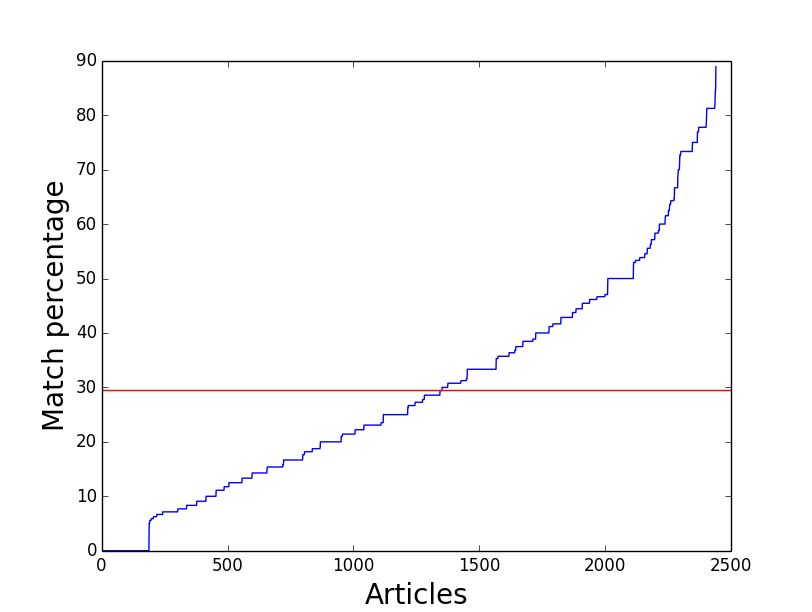
\includegraphics[width=0.5\textwidth, height=6cm]{unigrammatch}
\caption{Distribution of unigram match percentage over unique tweets and articles. Mean is 29.53\%, indicated by the red horizontal line, with a standard deviation of 20.2\%}
\label{fig:unigrammatch}
\end{figure}


\begin{figure}[tbp]
\centering
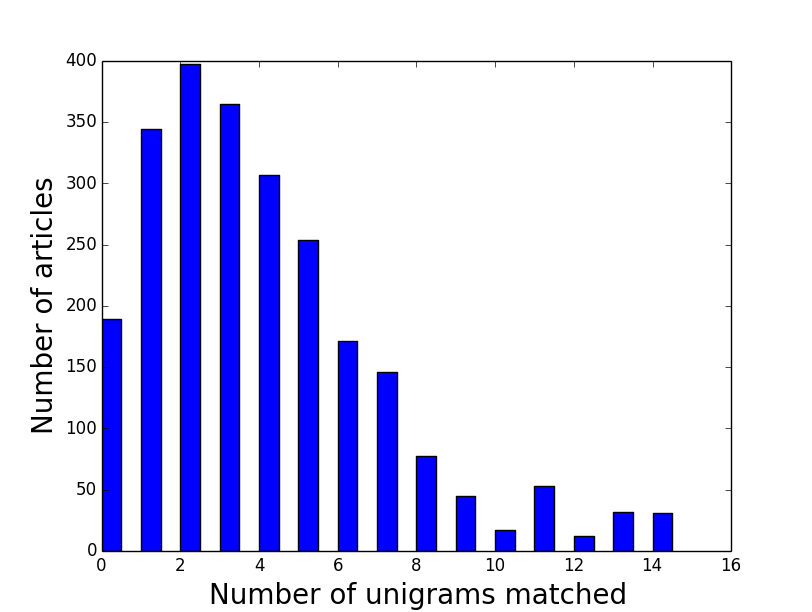
\includegraphics[width=0.5\textwidth, height=6cm]{num_unigrams}
\caption{Histogram of number of unique tweet-article pairs vs number of unigrams matched. The mean number of unigrams matched per tweet-article pair is 3.9.}
\label{fig:num_unigrams}
\end{figure}


\subsection{Percentage Match for Unigrams}
\label{sec:unigrams}

Next, we did a percentage match with the text of the article. This was a bag-of-words check using unigrams from the tweet and the document. Let $\textit{unigrams}(x)$ be the set of unigrams for some text $x$, then $u$, the percentage of matching unigrams found between a given tweet, $t$ and a given article, $a$, can be defined as  

\begin{equation}
u = \frac{| unigrams(t) \cap unigrams(a) |}{| unigrams(t) |} * 100
\end{equation}

\figref{fig:unigrammatch} shows the percentage of matches in the tweet and the article text as compared to the number of unigrams in the tweet. The mean match percentage is 29.53\% and standard deviation is 20.2\%. The mean of this distribution shows that the number of matched unigrams from a tweet in the article are fairly low. \figref{fig:num_unigrams} shows the number of articles with a certain number of matching unigrams. The graph shows that the most common number of unigrams matched was 2. The number of articles with higher unigrams matched goes on decreasing. The slight rise at the end - more than 10 matched unigrams - is accounted for by the completely matched tweets described above.

\begin{figure}[tbp]
\centering
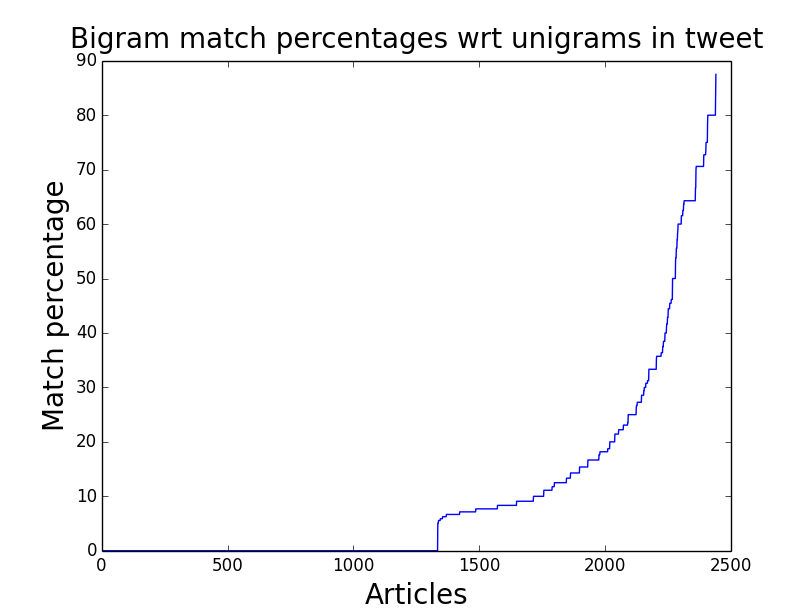
\includegraphics[width=0.5\textwidth, height=6cm]{bigrammatch}
\caption{Distribution of bigram match percentage over the tweet-article pair. The mean here is 10.73\% shown by the red horizontal line, with a standard deviation of 18.5\%}
\label{fig:bigrammatch}
\end{figure}


\subsection{Percentage Match for Bigrams}
\label{sec:bigrams}

Similar to the unigram matching techniques, the bigram percentage matching was also calculated. The text of the tweet was converted into bigrams and we then looked for those bigrams in the article text. The percentage was calculated similar to the unigram matching done earlier. For the set of bigrams for a text $x$, $\textit{bigrams}(x)$, percentage of matching bigrams $b$ for the tweet $t$ and article $a$ is: 

\begin{equation}
b = \frac{| bigrams(t) \cap bigrams(a) |}{| bigrams(t) |} * 100
\end{equation}

\figref{fig:bigrammatch} shows the percentages of matched bigrams found. The mean is 10.73 with a standard deviation of 18.5. As seen in the figure, most of the tweet-article pairs have no matched bigrams. The percentage then increases to reflect the complete matches found above.

\begin{figure}[tbp]
\centering
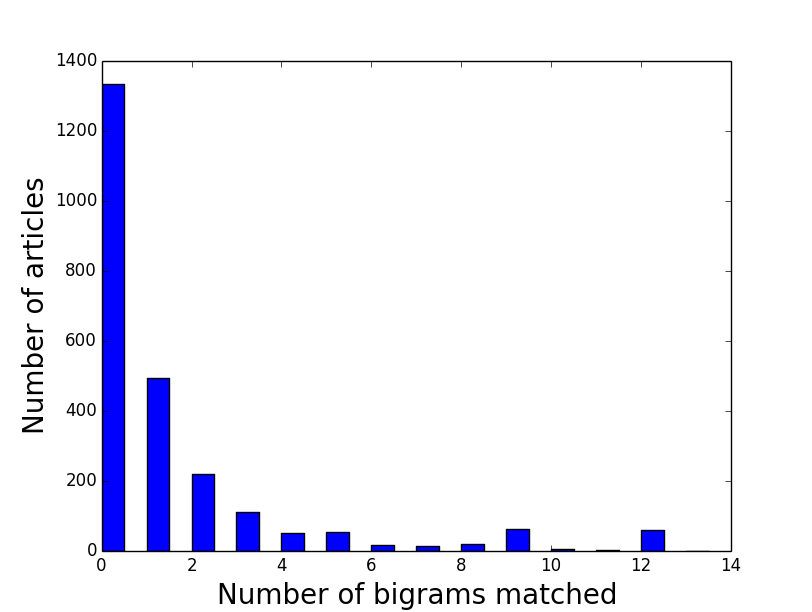
\includegraphics[width=0.5\textwidth, height=6cm]{num_bigrams}
\caption{Histogram of number of unique tweet-article pairs vs number of bigrams matched. The mean number of bigrams matched per article is 1.9.}
\label{fig:num_bigrams}
\end{figure}

\figref{fig:num_bigrams} shows frequency of the number of tweet-article pairs for the number of bigrams matched. There are no matched bigrams for most of the pairs. A smaller number of articles had one matched bigram, and the number decreased until the end, where it increases a little at more than 10 matched bigrams because of exact tweet matches. 


\subsection{Percentage Match Inside a Window in the Article Text}
\label{sec:window}

The next analysis checks for a significant word matching inside a three-sentence window inside the article text. We used a three sentence long window using the sentence boundary information obtained during preprocessing. A window of three sentences was chosen to give a smaller context for the tweet to be extracted from than the entire article. The number was chosen as a moderate context window size as not too small to reduce it to a sentence level, and not too big for the context to be diluted. This was done to investigate whether a pseudo-extractive sentence compression approach could convert a small number of sentences into a tweet.

After the text of the window was extracted, we performed a similar analysis as the last one, except on a smaller set of sentences. The matching percentages from all three-sentence windows in the articles were computed and the maximum out of these was taken for the final results. Let a sentence window $w_i$ be the set of three consecutive sentences starting from the sentence number $i$. For this window, the unigram match in the tweet $t$, and the window is the unigram match $u$ calculated above. Then, the maximum match from all the windows, $uw$ is 

\begin{equation}
uw = max_{w_i \in S} u(t, w_i)
\end{equation}

\begin{figure}[tbp]
\centering
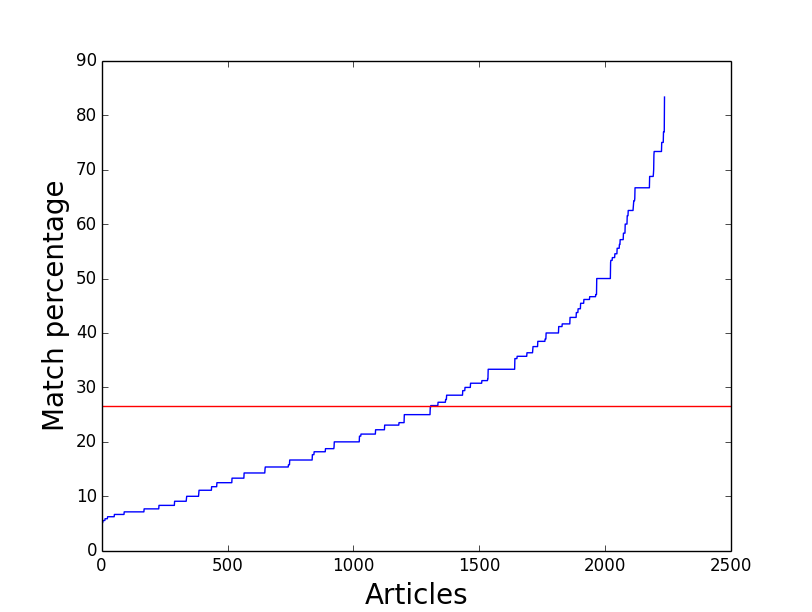
\includegraphics[width=0.5\textwidth, height=6cm]{unigramwindow}
\caption{Percentages of common words in tweet and a three sentence window in the article. The maximum match from all percentages is chosen for an article. The red horizontal line is the mean is 26.6\%, and standard deviation 17\%.}
\label{fig:unigramwindow}
\end{figure}

The result from this experiment is shown in \figref{fig:unigramwindow}. Here, the mean of the values is 26.6\% and deviation 17\%. Again this shows that only a small proportion of tweets can be generated even with an approach that combines unigrams from multiple sentences in the article.


\subsection{Longest Common Subsequence Match Inside a Window for the Text}
\label{sec:lcs}

The percentage match analyses were a bag-of-words approach that disregarded the order of the words inside the texts and tweets. To respect the order of the words in the sentence of the tweet, we also used the least common subsequence algorithm between the tweet text and the document text. This subsequence matching was done inside a sentence window of 5 sentences. 
Again, the final result for the article was the window in which the maximum percentage was recorded among all windows. The percentage match was calculated using the number of words in the tweet as the denominator.

If $\textit{lcs(t, a)}$ is the longest common subsequence between the tweet $t$ and article $a$, $\textit{unigrams}(x)$ is the set of unigrams for a text $x$, then the percentage of match for the lcs as compared to the tweet, $\textit{l}$ is



\begin{equation}
l = \frac{| lcs(t, a) |}{| unigrams(t) |} * 100
\end{equation}

\begin{figure}[tbp]
\centering
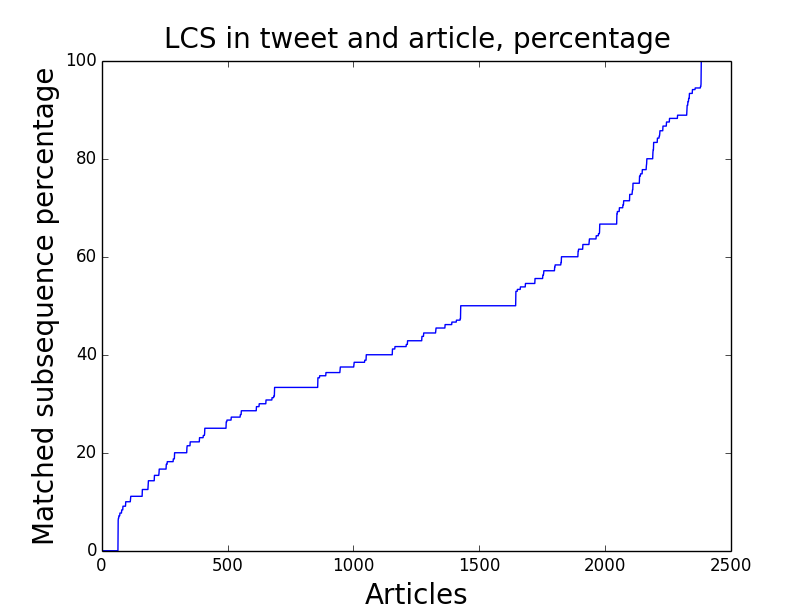
\includegraphics[width=0.5\textwidth, height=6cm]{lcs_doc}
\caption{Percentages of words matching in tweet and document text using an LCS algorithm. Mean is 44.6\%, which is shown by the red horizontal line, and standard deviation is 22.7\%.}
\label{fig:lcs}
\end{figure}

 These numbers are shown in \figref{fig:lcs}. The mean here is 44.6\% and the standard deviation is 22.7\%. 




\section{Interaction with Formality}

As seen in the results of the analyses performed in \secref{sec:analysis}, the tweets have little in common with the articles they are linked to. This shows that extractive summarization algorithms can only recover a small proportion of the indicative tweets. 

To tie in the results of the findings above with some intuitive notions about the text and see how formality interacts with the results, we also calculated the formality of the articles. This formality score was correlated with the longest common subsequence measure that we defined above. 

We assume that the formality of an article can be estimated by the formality of the words and phrases in the article. We used the formality lexicon of \newcite{brooke2013multi}. They calculate formality scores for words and sentences by training a model on a large corpus based on the appearance of words in specific documents. Their model represents words as vectors and the formal and informal seeds appear in opposite halves of the graphs, suggesting that we can use these seeds to determine if an article is formal or informal. The lexicon consists of words and phrases and their degree of formality. Thus, more formal words are marked on a positive scale and informal words like those occurring in colloquial language are marked on a negative scale. 

Let the set of formality expressions from the lexicon be $L$, and the formality score for an expression $e$ be $\textit{score}(e)$. Let the set of all substrings from the article $\textit{substrings}(a)$ be $S$. Then, the formality score $f$ for an article $a$ is the number of formal expressions per 10 words in article\todo{equation does not match this description. If it's per 10 words, the 10 should be in the denominator.}:  

\begin{equation}
f = \frac{\sum\limits_{e \in L, e \in S} \textit{score}(e)}{| unigrams(a) |} * 10
\end{equation}

The formality lexicon gave positive weights for formal expressions and negative for informal expressions. After calculating the formality weights for all articles, we observed that they all had a total negative normalized weight, meaning that many more informal expressions were getting matched. Hence, we used just the formal word occurrences for calculating the weight.\todo{I don't understand why this was a problem, and why we decided to only use the formal words...} As a check that these formality scores made intuitive sense, we calculated the average formality score for the articles belonging to each hashtag ordered them, as shown in \tabref{tab:formal}.


\begin{table}[htbp]
\centering
\begin{tabular}{|l|l|}
\hline
Lowest  & Highest  \\ \hline
\#theforceawakens       & \#KevinVickers           \\
\#TaylorSwift           & \#erdogan                \\
\#winteriscoming        & \#apec                  \\ \hline
\end{tabular}
\captionof{table}{Table of hashtags(broadly, topics) with highest and lowest formality according to the lexicon.}
\label{tab:formal}
\end{table}

This formality score for each article was correlated with the percentage of match obtained using the longest common subsequence algorithm. The Pearson correlation value was 0.41, with a p-value of 7.08e-66, indicating that the interaction between formality and overlap was highly significant. Hence, we can say that the more formal the subject or the article, the better that the tweet can be extracted from the article. \tabref{tab:formal} gives an example of the formality of the article, which is a low 4.2 formality words per 10 words, where the tweet is not extracted from the article, but rephrased from the article instead.

\begin{table}[htbp]
\centering
\begin{tabular}{|p{0.1\linewidth}|p{0.8\linewidth}|}
\hline
Tweet &  @globetoronto: Why Buffalo got clobbered with snow and Toronto did not. \#weather \#snowstorm http://t.co/gcwwoDPZmX... http://t.co/BXY7EH6F3u" \\ \hline
Title & What caused Buffalo’s massive snow and why Toronto got lucky \\  \hline
Text  & Torontonians have long been the butt of jokes about calling in the army every time a few snow flurries whip by... \\ \hline
\end{tabular}
\captionof{table}{Example of a tweet, title of the article where the formality of the article is over the mean, and the tweet is extracted from the article.}
\label{tab:formal}
\end{table}

\section{Discussions}
Having presented the above statistics showing that only a small portion of indicative tweets can be recovered from the article they link to if viewed as an extractive summarization problem, the question then becomes, how should we view the process of tweet generation?

We think that one promising direction is to model more explicitly the intent, or the purpose of the tweets. There have been several studies on classifying intents in tweets, but in many cases the intents are general, high-level intents of the tweets, more akin to classifying the topic or genre of the tweet than the intent. \newcite{wang2015mining} classify intents as food and drink, travel, career and so on, ones that can directly be used as intents for purchasing and can be utilized for advertisements. They also focus on finding tweets with intent and then classifying those. \newcite{banerjee2012towards} analyze real time data to detect presence of intents in tweets. \newcite{gomez2014content} use features from text and stylistics to determine user intentions, which are classified as news report, opinion, publicity and so on. \newcite{mohammad2013identifying} study the classification of user intents specifically for tweets related to elections. They study one election and classify tweets as ones that agree or disagree with the candidate, ones that are meant for humour, support and so on. 

These definitions of intent, while a promising start, will not be sufficient for tweet generation. For this purpose, intent would be the reason the user chose to share the article with that particular text. This would include reasons like support some cause, promote a product or an article, agree or disagree with an event, or express an opinion about it. Identifying these intents will help provide parameters for generating tweets. 


\section{Conclusion}
\todo{Write}

However, after running analyses on the data we discovered that it does not make sense to model tweet generation from articles as an extractive summarization problem. The size of the tweet is too small to be able to form a coherent sentence for the tweet.


%\section*{Acknowledgments}
% We would like to thank Julian Brooke for providing us with his formality lexicon.

% include your own bib file like this:
\bibliographystyle{acl}
\bibliography{acl2015}

\end{document}